\section{Background and Related Work}
\label{sec:background}

\subsection{Decision and Regression Trees}

A Decision Tree recursively partitions the feature space using binary questions
on single features (e.g., $\texttt{sqft\_living} \leq 2915$), storing a
prediction at each leaf~\cite{breiman1984cart}. Trees handle mixed feature
types, need no scaling, and are interpretable, but a single tree is unstable and
overfits easily---motivating the ensembles below. For a continuous target the
tree becomes a \textbf{regression tree}: rather than fitting one global formula
(as linear regression does), it partitions the space into local regions and
predicts the sample mean in each~\cite{hastie2009elements}. Letting $S$ be the
samples reaching a node, the chosen split maximises the reduction in sum of
squared errors and each leaf $S_{\ell}$ predicts the mean:
\begin{equation}
  \Delta\text{SSE} = \text{SSE}(S) - \text{SSE}(S_L) - \text{SSE}(S_R),
  \quad \text{SSE}(S) = \sum_{i \in S}(y_i - \bar{y}_S)^2,
  \quad \hat{y}_{\ell} = \frac{1}{|S_{\ell}|}\sum_{i \in S_{\ell}} y_i.
\end{equation}
Because features such as \texttt{sqft\_living}, \texttt{waterfront}, and
\texttt{view} interact non-linearly, a regression tree is a natural baseline here.

\subsection{Gradient Boosting and Random Forests}

Gradient Boosting~\cite{friedman2001greedy} combines many \emph{shallow} trees
additively, building the ensemble stage by stage so that each new tree corrects
the current residual:
\begin{equation}
  F_K(x) = F_0(x) + \eta\sum_{k=1}^{K} h_k(x),
  \qquad r_i^{(k)} = y_i - F_{k-1}(x_i),
\end{equation}
where $F_0$ is an initial prediction, $\eta$ the learning rate, and $h_k$ fits
the negative gradient (the residual for squared error). A common refinement,
\emph{stochastic gradient boosting}, fits each tree on a random
subsample to reduce variance~\cite{friedman2002stochastic}; the XGBoost modules
used in our mGBDT support this.

A \textbf{Random Forest}~\cite{breiman1984cart} instead reduces variance by
\emph{bagging}: it trains many trees on bootstrap resamples and considers a
random feature subset at each split, so averaging the de-correlated trees cancels
per-tree noise. Being robust and low-tuning, a Random Forest on the naively
(ordinal) encoded categories serves as our baseline.

\subsection{Multi-Layered Gradient Boosting Decision Trees}

Standard GBDTs learn a \emph{flat} ensemble---all trees share one input
representation---whereas deep networks learn \emph{hierarchical} representations
through stacked layers. The mGBDT framework~\cite{feng2018mgbdt} bridges this gap
by stacking $M$ GBDT modules, the output of layer $l$ feeding layer $l+1$
($o_0=x$, $o_l = F_l(o_{l-1})$). Since GBDTs are non-differentiable, mGBDT
replaces back-propagation with \emph{target propagation}: the final layer is
trained toward $y$, and inverse mappings $G_l$ propagate pseudo-labels backward
($\tilde{o}_{l-1} = G_l(\tilde{o}_l)$, $\tilde{o}_M = y$) so each layer $F_l$
receives its own target. The project hypothesis is that this layered
representation captures hierarchical feature interactions better than a flat GBDT.

\begin{figure}[h]
\centering
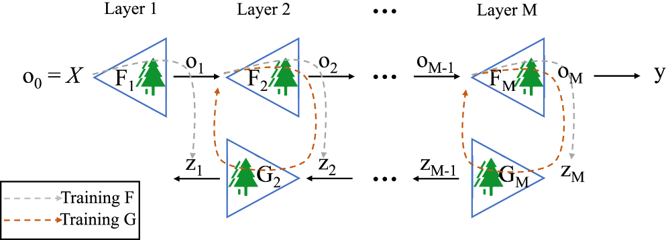
\includegraphics[width=0.95\textwidth]{results/mgbdt.png}
\caption{mGBDT architecture}
\label{fig:mgbdt_architecture}
\end{figure}

We instantiate $F_l$ and $G_l$ with XGBoost~\cite{chen2016xgboost} modules. A
two-layer mGBDT was tried, but its second layer learned noise and
\emph{degraded} accuracy (Section~\ref{sec:result}); the single-layer
configuration we report---one target-propagation layer over XGBoost---reduces to
standard gradient boosting, so our ``mGBDT'' results are effectively those of
plain XGBoost, which we adopt as the final boosting model.
